\documentclass[12pt, titlepage]{article}

\usepackage{fullpage}
\usepackage[round]{natbib}
\usepackage{multirow}
\usepackage{booktabs}
\usepackage{tabularx}
\usepackage{graphicx}
\usepackage{float}
\usepackage{hyperref}
\hypersetup{
    colorlinks,
    citecolor=blue,
    filecolor=black,
    linkcolor=red,
    urlcolor=blue
}

\input{../../Comments}
\input{../../Common}

\newcounter{acnum}
\newcommand{\actheacnum}{AC\theacnum}
\newcommand{\acref}[1]{AC\ref{#1}}

\newcounter{ucnum}
\newcommand{\uctheucnum}{UC\theucnum}
\newcommand{\uref}[1]{UC\ref{#1}}

\newcounter{mnum}
\newcommand{\mthemnum}{M\themnum}
\newcommand{\mref}[1]{M\ref{#1}}

\begin{document}

\title{Module Guide for \progname{}} 
\author{\authname}
\date{\today}

\maketitle

\pagenumbering{roman}

\section{Revision History}

\begin{tabularx}{\textwidth}{p{3cm}p{2cm}X}
\toprule {\bf Date} & {\bf Version} & {\bf Notes}\\
\midrule
Date 1 & 1.0 & Notes\\
Date 2 & 1.1 & Notes\\
\bottomrule
\end{tabularx}

\newpage

\section{Reference Material}

This section records information for easy reference.

\subsection{Abbreviations and Acronyms}

\renewcommand{\arraystretch}{1.2}
\begin{tabular}{l l} 
  \toprule		
  \textbf{symbol} & \textbf{description}\\
  \midrule 
  AC & Anticipated Change\\
  DAG & Directed Acyclic Graph \\
  M & Module \\
  MG & Module Guide \\
  OS & Operating System \\
  R & Requirement\\
  SC & Scientific Computing \\
  SRS & Software Requirements Specification\\
  \progname & Explanation of program name\\
  UC & Unlikely Change \\
  \wss{etc.} & \wss{...}\\
  \bottomrule
\end{tabular}\\

\newpage

\tableofcontents

\listoftables

\listoffigures

\newpage

\pagenumbering{arabic}

\section{Introduction}

Decomposing a system into modules is a commonly accepted approach to developing
software.  A module is a work assignment for a programmer or programming
team~\citep{ParnasEtAl1984}.  We advocate a decomposition
based on the principle of information hiding~\citep{Parnas1972a}.  This
principle supports design for change, because the ``secrets'' that each module
hides represent likely future changes.  Design for change is valuable in SC,
where modifications are frequent, especially during initial development as the
solution space is explored.  

Our design follows the rules layed out by \citet{ParnasEtAl1984}, as follows:
\begin{itemize}
\item System details that are likely to change independently should be the
  secrets of separate modules.
\item Each data structure is implemented in only one module.
\item Any other program that requires information stored in a module's data
  structures must obtain it by calling access programs belonging to that module.
\end{itemize}

After completing the first stage of the design, the Software Requirements
Specification (SRS), the Module Guide (MG) is developed~\citep{ParnasEtAl1984}. The MG
specifies the modular structure of the system and is intended to allow both
designers and maintainers to easily identify the parts of the software.  The
potential readers of this document are as follows:

\begin{itemize}
\item New project members: This document can be a guide for a new project member
  to easily understand the overall structure and quickly find the
  relevant modules they are searching for.
\item Maintainers: The hierarchical structure of the module guide improves the
  maintainers' understanding when they need to make changes to the system. It is
  important for a maintainer to update the relevant sections of the document
  after changes have been made.
\item Designers: Once the module guide has been written, it can be used to
  check for consistency, feasibility and flexibility. Designers can verify the
  system in various ways, such as consistency among modules, feasibility of the
  decomposition, and flexibility of the design.
\end{itemize}

The rest of the document is organized as follows. Section
\ref{SecChange} lists the anticipated and unlikely changes of the software
requirements. Section \ref{SecMH} summarizes the module decomposition that
was constructed according to the likely changes. Section \ref{SecConnection}
specifies the connections between the software requirements and the
modules. Section \ref{SecMD} gives a detailed description of the
modules. Section \ref{SecTM} includes two traceability matrices. One checks
the completeness of the design against the requirements provided in the SRS. The
other shows the relation between anticipated changes and the modules. Section
\ref{SecUse} describes the use relation between modules.

\section{Anticipated and Unlikely Changes} \label{SecChange}

This section lists possible changes to the system. According to the likeliness
of the change, the possible changes are classified into two
categories. Anticipated changes are listed in Section \ref{SecAchange}, and
unlikely changes are listed in Section \ref{SecUchange}.

\subsection{Anticipated Changes} \label{SecAchange}

Anticipated changes are the source of the information that is to be hidden
inside the modules. Ideally, changing one of the anticipated changes will only
require changing the one module that hides the associated decision. The approach
adapted here is called design for
change.

\begin{description}
\item[\refstepcounter{acnum} \actheacnum \label{acLayout}:] The layout and order of prompts or screens that are presented during the user registration process.
\item[\refstepcounter{acnum} \actheacnum \label{acDiscovery}:] The process by which users discover new content / other users.
\item[\refstepcounter{acnum} \actheacnum \label{acStorage}:] Leverage local storage for exercises and workouts instead of storing all data on database. 
\item[\refstepcounter{acnum} \actheacnum \label{acStyling}:] Visual styling and color design choices.
\end{description}

\subsection{Unlikely Changes} \label{SecUchange}

The module design should be as general as possible. However, a general system is
more complex. Sometimes this complexity is not necessary. Fixing some design
decisions at the system architecture stage can simplify the software design. If
these decision should later need to be changed, then many parts of the design
will potentially need to be modified. Hence, it is not intended that these
decisions will be changed.

\begin{description}
\item[\refstepcounter{ucnum} \uctheucnum \label{ucLegal}:] Security requirements and legal compliance requirements are unlikely to be changed: NFR15, NFR16, NFR17, NFR18, NFR22.
\item[\refstepcounter{ucnum} \uctheucnum \label{ucUsability}:] To maintain accessibility for all users, the following Usability and Humanity requirements are likely to remain unchanged: NFR2, NFR3, NFR4, NFR5, NFR6, NFR7.
\item[\refstepcounter{ucnum} \uctheucnum \label{ucPerformance}:] The performance requirement specified by NFR8 encapsulates the mission of this application, which is to allow users to quickly update / interact with programs. As such, it is unlikely to change.
\end{description}

\section{Module Hierarchy} \label{SecMH}

This section provides an overview of the module design. Modules are summarized
in a hierarchy decomposed by secrets in Table \ref{TblMH}. The modules listed
below, which are leaves in the hierarchy tree, are the modules that will
actually be implemented.

\begin{description}
\item [\refstepcounter{mnum} \mthemnum \label{mHH}:] Hardware-Hiding Module
\item [\refstepcounter{mnum} \mthemnum \label{mExercise}:] Exercise Module
\item [\refstepcounter{mnum} \mthemnum \label{mWorkout}:] Workout Module
\item [\refstepcounter{mnum} \mthemnum \label{mWR}:] Workout Routine Module
\item [\refstepcounter{mnum} \mthemnum \label{mUL}:] User Login Module
\item [\refstepcounter{mnum} \mthemnum \label{mUR}:] User Registration Module
\item [\refstepcounter{mnum} \mthemnum \label{mUP}:] User Profile Module
\item [\refstepcounter{mnum} \mthemnum \label{mUFG}:] User Fitness Goal Module
\item [\refstepcounter{mnum} \mthemnum \label{mWB}:] User Workout Browser Module
\item [\refstepcounter{mnum} \mthemnum \label{mCreation}:] Creation Module
\item [\refstepcounter{mnum} \mthemnum \label{mWC}:] Workout Creation Module
\item [\refstepcounter{mnum} \mthemnum \label{mWRC}:] Workout Routine Creation Module
\item [\refstepcounter{mnum} \mthemnum \label{mEC}:] Exercise Creation Module
\item [\refstepcounter{mnum} \mthemnum \label{mTS}:] Timed Sequence Module
\item [\refstepcounter{mnum} \mthemnum \label{mQuantifier}:] Quantifier Module
\end{description}


\begin{table}[h!]
\centering
\begin{tabular}{p{0.3\textwidth} p{0.6\textwidth}}
\toprule
\textbf{Level 1} & \textbf{Level 2}\\
\midrule

{Hardware-Hiding Module} & ~ \\
\midrule

\multirow{12}{0.3\textwidth}{Behaviour-Hiding Module}
& exercise\\
& workout\\
& workout routine\\
& user login\\
& user registration\\
& user profile\\ 
& user fitness goal\\
& workout browser\\
& creation\\
& workout creation\\
& workout routine creation\\
& exercise creation\\
& timed sequence\\
\midrule

\multirow{1}{0.3\textwidth}{Software Decision Module}
& quantifier\\
\bottomrule

\end{tabular}
\caption{Module Hierarchy}
\label{TblMH}
\end{table}

\section{Connection Between Requirements and Design} \label{SecConnection}

The design of the system is intended to satisfy the requirements developed in
the SRS. In this stage, the system is decomposed into modules. The connection
between requirements and modules is listed in Table \ref{TblRT}.

\section{Module Decomposition} \label{SecMD}

Modules are decomposed according to the principle of ``information hiding''
proposed by \citet{ParnasEtAl1984}. The \emph{Secrets} field in a module
decomposition is a brief statement of the design decision hidden by the
module. The \emph{Services} field specifies \emph{what} the module will do
without documenting \emph{how} to do it. For each module, a suggestion for the
implementing software is given under the \emph{Implemented By} title. If the
entry is \emph{OS}, this means that the module is provided by the operating
system or by standard programming language libraries.  \emph{\progname{}} means the
module will be implemented by the \progname{} software.

Only the leaf modules in the hierarchy have to be implemented. If a dash
(\emph{--}) is shown, this means that the module is not a leaf and will not have
to be implemented.

\subsection{Hardware Hiding Modules (\mref{mHH})}

\begin{description}
\item[Secrets:]The data structure and algorithm used to implement the virtual
  hardware.
\item[Services:]Serves as a virtual hardware used by the rest of the
  system. This module provides the interface between the hardware and the
  software. So, the system can use it to display outputs or to accept inputs.
\item[Implemented By:] OS
\end{description}

\subsection{Behaviour-Hiding Module}

\begin{description}
\item[Secrets:]The contents of the required behaviours.
\item[Services:]Includes programs that provide externally visible behaviour of
  the system as specified in the software requirements specification (SRS)
  documents. This module serves as a communication layer between the
  hardware-hiding module and the software decision module. The programs in this
  module will need to change if there are changes in the SRS.
\item[Implemented By:] --
\end{description}

\subsubsection{Exercise Module (\mref{mExercise})}

\begin{description}
\item[Secrets:] The values of quantifiers and descriptions for each exercise.
\item[Services:] Provides read and write (get and set) capability for individual exercises.
\item[Implemented By:] exercise.ts
\item[Type of Module:] Abstract Object
\end{description}

\subsubsection{Workout Module (\mref{mWorkout})}

\begin{description}
\item[Secrets:] The exercises that make up each workout.
\item[Services:] Manage (read and write) which exercises comprise a workout.
\item[Implemented By:] workout.ts
\item[Type of Module:] Abstract Object
\end{description}

\subsubsection{Workout Routine Module (\mref{mWR})}

\begin{description}
\item[Secrets:] The workouts and scheduling to make up a workout routine.
\item[Services:] Manage the scheduling and contents of a workout routine.
\item[Implemented By:] workout-routine.ts
\item[Type of Module:] Abstract Object
\end{description}

\subsubsection{User Login Module (\mref{mUL})}

\begin{description}
\item[Secrets:] The functions needed to verify a users identity. 
\item[Services:] Accepts user credentials and, if correct, provides a token to log user in.
\item[Implemented By:] user-login.ts
\end{description}

\subsubsection{User Registration Module (\mref{mUR})}

\begin{description}
\item[Secrets:] The functions needed to create a new user in the application database. 
\item[Services:] Accepts user credential data and, if valid, creates a new user in the database with the provided data.
\item[Implemented By:] user-registration.ts
\end{description}

\subsubsection{User Profile Module (\mref{mUP})}

\begin{description}
\item[Secrets:] The personal data for a user.
\item[Services:] Manage all personal user data.
\item[Implemented By:] user-profile.ts
\end{description}

\subsubsection{User Fitness Goal Module (\mref{mUFG})}

\begin{description}
\item[Secrets:] The quantifiers that users set for their fitness goals.
\item[Services:] Manage fitness goals for a specific user.
\item[Implemented By:] user-fitness-goals.ts
\end{description}

\subsubsection{Workout Browser Module (\mref{mWB})}

\begin{description}
\item[Secrets:] The data structure for filtering and displaying public workouts.
\item[Services:] Display public workouts and allow user to search and filter options.
\item[Implemented By:] workout-browser.ts
\end{description}

\subsubsection{Creation Module (\mref{mCreation})}

\begin{description}
\item[Secrets:] Abstract data type that provides children with methods for adding entries to the database.
\item[Services:] Provides general append functionality to database.
\item[Implemented By:] creation.ts
\end{description}

\subsubsection{Workout Creation Module (\mref{mWC})}

\begin{description}
\item[Secrets:] The verification of new workout data.
\item[Services:] Uses creation module to add new workout to database.
\item[Implemented By:] workout-creation.ts
\end{description}

\subsubsection{Workout Routine Creation Module (\mref{mWRC})}

\begin{description}
\item[Secrets:] The verification of new workout routine data.
\item[Services:] Uses creation module to add new workout routine to database.
\item[Implemented By:] workout-routine-creation.ts
\end{description}

\subsubsection{Exercise Creation Module (\mref{mEC})}

\begin{description}
\item[Secrets:] The verification of new exercise data.
\item[Services:] Uses creation module to add new exercise to database.
\item[Implemented By:] exercise-creation.ts
\end{description}

\subsubsection{Timed Sequence Module (\mref{mTS})}

\begin{description}
\item[Secrets:] A general format and structure of sequence data
\item[Services:] Provides methods to access and create timed sequences.
\item[Implemented By:] timed-sequence.ts
\end{description}

\subsection{Software Decision Module}

\begin{description}
\item[Secrets:] The design decision based on mathematical theorems, physical
  facts, or programming considerations. The secrets of this module are
  \emph{not} described in the SRS.
\item[Services:] Includes data structure and algorithms used in the system that
  do not provide direct interaction with the user. 
  % Changes in these modules are more likely to be motivated by a desire to
  % improve performance than by externally imposed changes.
\item[Implemented By:] --
\end{description}

\subsubsection{Quantifier Module (\mref{mQuantifier})}
\begin{description}
\item[Secrets:] The data types used to quantify workout exercises.
\item[Services:] Measures the exercise inputted by users as a unit of measurement.
\item[Implemented By:] quantifiers.ts
\item[Type of Module:] Abstract Data Type
\end{description}

\section{Traceability Matrix} \label{SecTM}

This section shows two traceability matrices: between the modules and the
requirements and between the modules and the anticipated changes.

% the table should use mref, the requirements should be named, use something
% like fref
\begin{table}[H]
\centering
\begin{tabular}{p{0.2\textwidth} p{0.6\textwidth}}
\toprule
\textbf{Req.} & \textbf{Modules}\\
\midrule
FR1 & \mref{mWRC}\\
FR2 & \mref{mExercise}, \mref{mWR}, \mref{mEC}\\
FR3 & \mref{mExercise}, \mref{mQuantifier}\\
FR4 & \mref{mWR}, \mref{mUP}\\
FR5 & \mref{mWR}\\
FR6 & \mref{mWR}, \mref{mWB}\\
FR7 & \mref{mUP}\\
FR8 & \mref{mUP}\\
FR9 & \mref{mExercise}, \mref{mUFG}, \mref{mEC}, \mref{mQuantifier}\\
FR10 & \mref{mExercise}, \mref{mUFG}, \mref{mQuantifier}\\
FR11 & \mref{mUFG}, \mref{mWB}\\

\bottomrule
\end{tabular}
\caption{Trace Between Requirements and Modules}
\label{TblRT}
\end{table}

\begin{table}[H]
\centering
\begin{tabular}{p{0.2\textwidth} p{0.6\textwidth}}
\toprule
\textbf{AC} & \textbf{Modules}\\
\midrule
\acref{acLayout} & \mref{mUR}\\
\acref{acDiscovery} & \mref{mWB}\\
\acref{acStorage} & \mref{mHH}\\
\acref{acStyling} & \mref{mWorkout}\\
\bottomrule
\end{tabular}
\caption{Trace Between Anticipated Changes and Modules}
\label{TblACT}
\end{table}

\section{Use Hierarchy Between Modules} \label{SecUse}

In this section, the uses hierarchy between modules is
provided. \citet{Parnas1978} said of two programs A and B that A {\em uses} B if
correct execution of B may be necessary for A to complete the task described in
its specification. That is, A {\em uses} B if there exist situations in which
the correct functioning of A depends upon the availability of a correct
implementation of B.  Figure \ref{FigUH} illustrates the use relation between
the modules. It can be seen that the graph is a directed acyclic graph
(DAG). Each level of the hierarchy offers a testable and usable subset of the
system, and modules in the higher level of the hierarchy are essentially simpler
because they use modules from the lower levels.

\begin{figure}[H]
\centering
%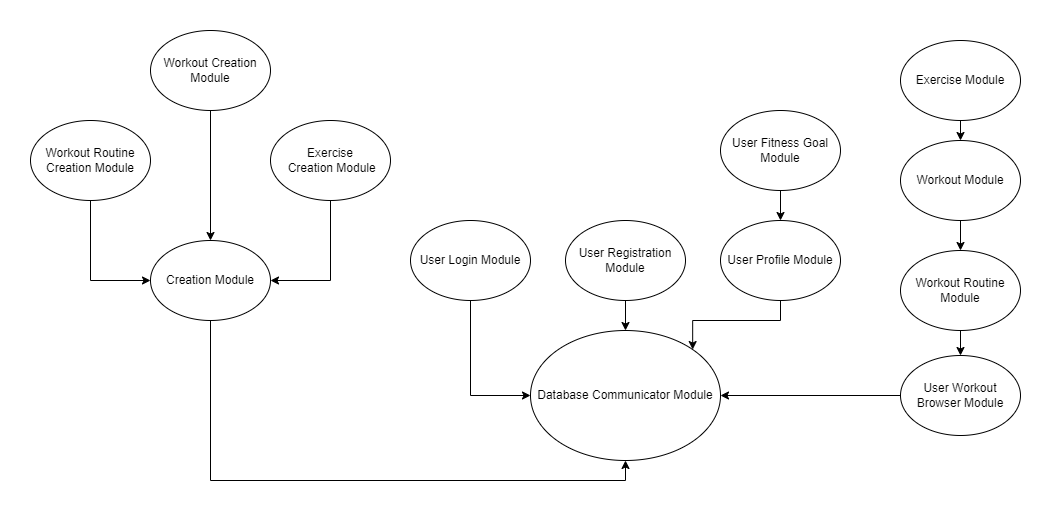
\includegraphics[width=0.7\textwidth]{UsesHierarchy.png}
\caption{Use hierarchy among modules}
\label{FigUH}
\end{figure}

%\section*{References}

\bibliographystyle {plainnat}
\bibliography{../../../refs/References}

\newpage{}
\section*{Appendix --- Reflection}

The information in this section will be used to evaluate the team members on the
graduate attribute of Lifelong Learning.  Please answer the following questions:

\begin{enumerate}
  \item 
  \item 
\end{enumerate}

\end{document}